\subsubsection{Database}
The persistence layer must include a DBMS component, in order to manage the insertion, modification, deletion of data and managing the relative transactions on the database.\\
Regardless of the implementation, the DBMS must guarantee the correct functioning of concurrent transactions and the ACID properties; it also must be a relational DBMS, since the application needs in terms of data storage do not require a more complex structure than the simple one provided by the relational data structure.\\
The data layer must only be accessible through the Application Server via a dedicated interface. With respect to this, the Application Server must provide a persistence unit to handle the dynamic behaviour of all of the persistent application data.\\
Sensible data such as passwords and personal information must be encrypted properly before being stored. Users must be granted access only upon provision of correct and valid credentials.\\
The E-R diagram illustrates a detailed view over the database schemas and attributes.

\begin{figure}[H]
\begin{center}
		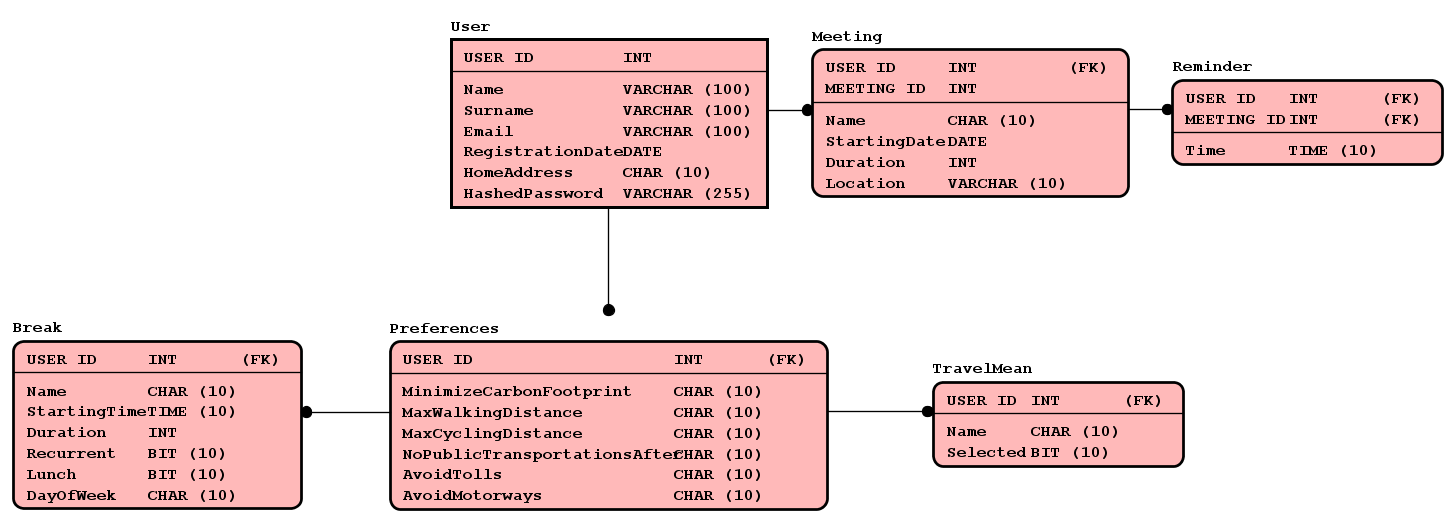
\includegraphics[width=1.3\textwidth]{images/ertravlendar}
		\caption{The E-R diagram of the database schema.}
		\label{erdiagram}
\end{center}
\end{figure}

\clearpage
We also provide a projection of the E-R diagram in the form of a class diagram:

\begin{figure}[H]
\begin{center}
		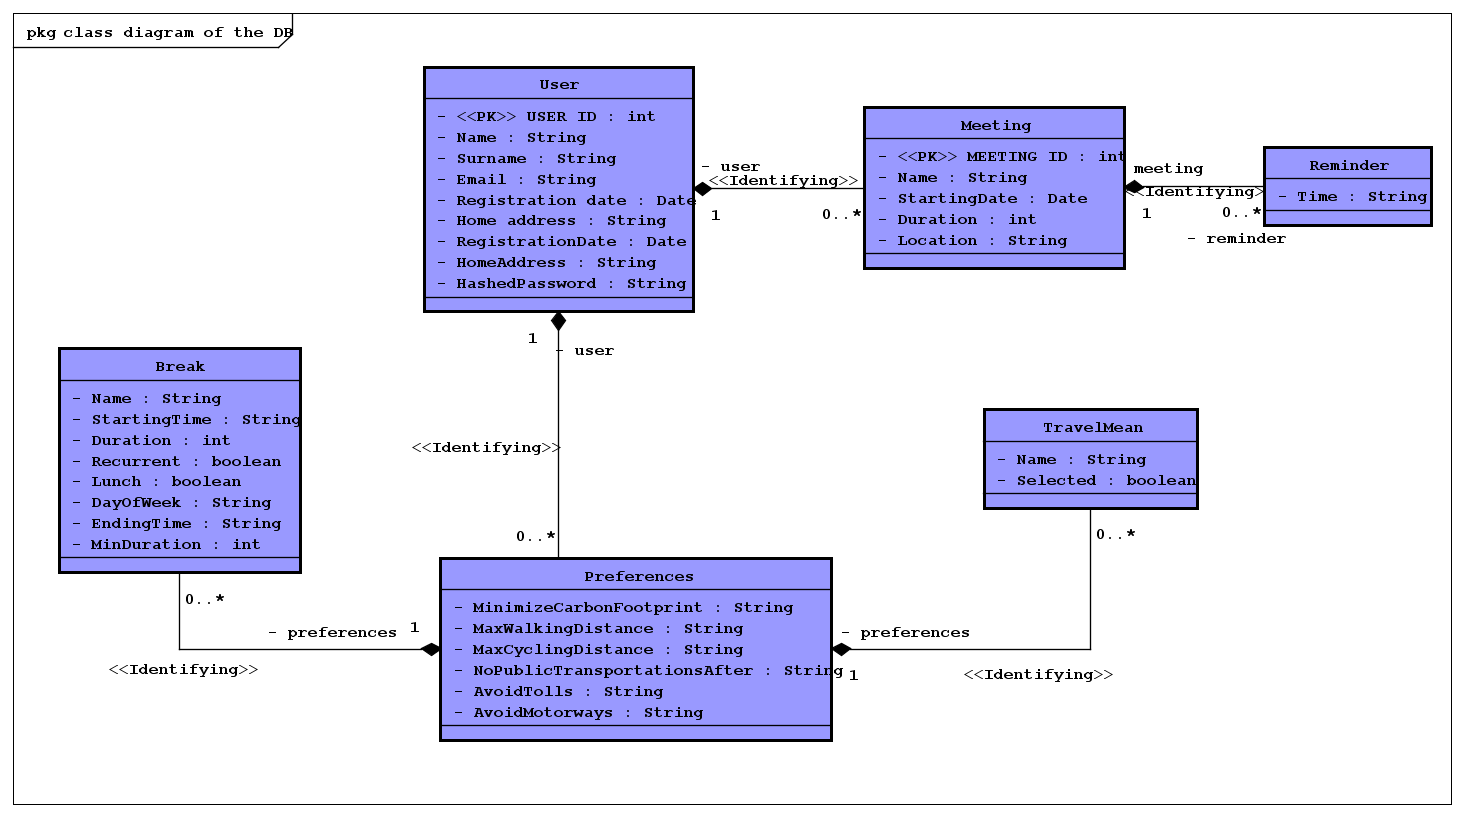
\includegraphics[width=1.3\textwidth]{images/databasedesignclass}
		\caption{The E-R diagram of the database schema.}
		\label{erdiagram}
\end{center}
\end{figure}


